\documentclass[letterpaper,10pt]{book}
% Change to 10 pt
\usepackage{pdfpages}
\usepackage{morewrites}			% to counteract the no write space problem
\setcounter{tocdepth}{6}

\usepackage[framemethod=TikZ]{mdframed}

\usepackage{fancyhdr}

\usepackage{paralist}
\usepackage{amsmath}
\usepackage{amsfonts}
\usepackage{amssymb}
\usepackage{graphicx}

\usepackage{datetime}
%\usepackage{ulem}

%\usepackage[nottoc]{toobibind}

\usepackage[inline]{enumitem}

% Outer margin at 2.50 is exacty correct to fit the ``corruption alert'' tables
\usepackage[inner=1.0in, outer=2.50in, top=2.54cm,bottom=2.54cm, marginparwidth=2.25in]{geometry}

\usepackage{marginnote}
\usepackage{longtable}
\usepackage{booktabs}
\usepackage{xcolor}

\usepackage{soul}

%%%%%%%%%%%%
\definecolor{ForestGreen}{rgb}{0.00,0.29,0.098}
%%%%%%%%%%%%

\usepackage{marginnote}

\usepackage{imakeidx} 
\usepackage[
	backref=true,
	style=numeric,
%	citestyle=numeric,
	backend=bibtex
	]{biblatex}
\usepackage[driverfallback=hypertex,colorlinks=True]{hyperref}
\usepackage{cleveref}

\makeindex[name=scripture,columnsep=20pt, columnseprule=True,columns=3, title=Scripture References]
\makeindex[name=speaker,columnsep=20pt, columnseprule=True,,columns=2, title=Sermon Creator]
\makeindex[name=series,columnsep=20pt, columnseprule=True,,columns=2, title=Sermon Series]
\makeindex[name=date,columnsep=20pt, columnseprule=True,columns=2, title=Sermon Date]
\makeindex[name=event,columnsep=20pt, columnseprule=True,columns=2, title=Event]
\makeindex[name=topic,columnsep=20pt, columnseprule=True,columns=2, title=Topic]
\makeindex[name=AWIP,columnsep=20pt, columnseprule=True,columns=3, title=All Words in Passage]
\makeindex[name=NWIV,columnsep=20pt, columnseprule=True,columns=3, title=Number of Words in Verse]
\makeindex[name=PNIP,columnsep=20pt, columnseprule=True,columns=3, title=Proper Names in Passage]
\makeindex[name=PEIP,columnsep=20pt, columnseprule=True,columns=2, title=Prophetic Events in Passage]
\makeindex[name=TWPAQ,columnsep=20pt, columnseprule=True,columns=1, title=13-Word Phrases and Quotes]
\makeindex[name=PFTTIS,columnsep=20pt, columnseprule=False,columns=3, title=Phrases found 13 times in scripture]
\makeindex[name=WFTTIS,columnsep=20pt, columnseprule=False,columns=3, title=Words found 13 times in scripture]
\makeindex[name=WFITV,columnsep=20pt, columnseprule=False,columns=3, title=Words found in exactly 13 verses]
\makeindex[name=EVENTS,columnsep=20pt, columnseprule=False,columns=2, title=Sermon Log by Place]
\makeindex[name=QUESTIONS,columnsep=20pt, columnseprule=False,columns=2, title=Bible Questions]
\makeindex[name=DOCTRINES,columnsep=20pt, columnseprule=False,columns=2, title=Doctrines]
\makeindex[name=SONGS,columnsep=20pt, columnseprule=False,columns=1, title=Songs]
\makeindex[name=LOCATION,columnsep=20pt, columnseprule=False,columns= 2, title=Location]
\makeindex[name=FACEBOOK,columnsep=20pt, columnseprule=False,columns=2, title=Facebook]
\makeindex[name=DEVOTIONAL,columnsep=20pt, columnseprule=False,columns=2, title=Devotional Items]
%%%%%%%%%%%%%%%%% EXTRA COLORS
\definecolor{champagne}{rgb}{0.97,0.91,0.81}
\definecolor{bone}{rgb}{0.89,0.85,0.79}
\pagestyle{fancy}
\fancyhf{}
\fancyhead[LE,RO]{\today}
\fancyhead[RE,LO]{Daily Bible Reading}
\fancyhead[CE,CO]{-page \thepage  - }

\fancyfoot[CO,CE]{\leftmark}
%\fancyfoot[LE,RO]{CSCE 692, HW1}

\title{DBR\\
Daily \\ Reads}
\author{Keith Anthony \\
\today }
%+/ffffff +   \pagenumbering{gobble}
\bibliography{Bibliographies/All20220122}

\setlength{\fboxsep}{1.0pt}

\usepackage[utf8]{inputenc}
\usepackage{tikz}

\begin{document}
%%%%%%%%%%%% Tile Page

\begin{titlepage}

\begin{flushright}
\rightskip=-2.5cm
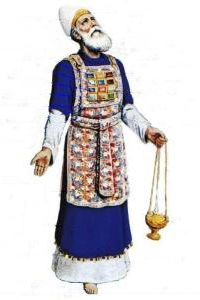
\includegraphics[width=50mm,scale=1.5]{Extras/Melchisedec.jpg}
\vspace{0.4in}  % Create a title for the document and write it in bold font
\LARGE{\textbf{\date}} % Again, do a line break
\linebreak 
% Create a subtitle \large{with Outlines, Statistics, Cross References, and Notes}
\vspace{0.5in}
\begin{flushleft}
\LARGE{Day \#71: Saturday, 12 March 2022 PLAIN \\}\vspace{0.25in}
\LARGE{Joshua 19-21 Psalm 71 Proverb 12}
\end{flushleft}
\vspace{0.6in}
\bigskip

\normalsize{Xenia, Oh.\\}
\normalsize{created: \today}
\vspace{1.3in}

\end{flushright}
\end{titlepage}

\newpage 
\tableofcontents\hypertarget{TOC}{}
\listoffigures
\listoftables

\hyphenation{A-bim-e-lech bre-thren E-phra-im  Gib-e-o-nites Jer-u-sa-lem through-out Phil-i-stines The-o-phil-us Am-a-le-kites ven-geance Mesh-el-e-mi-ah onan-ism Phar-a-oh thoughts grev-ous-ness Hach-a-liah adul-ter-er Shad-rach}

%%%%%%%%%%%%%%%%% EXTRA COLORS
%%%%%%%%%%%%%%%%% EXTRA COLORS
%%%%%%%%%%%%%%%%% EXTRA COLORS
\definecolor{champagne}{rgb}{0.97,0.91,0.81}
\definecolor{bone}{rgb}{0.89,0.85,0.79}

\definecolor{ForestGreen}{rgb}{0.00,0.29,0.098}
\definecolor{GIVING}{cmyk}{1,0.0,0.72,.1}

\definecolor{MLPE}{cmyk}{1,1,0,.45}
\definecolor{SOCCER}{cmyk}{.77, 0, .42, .49}
\definecolor{PAYBILL}{cmyk}{0,0.83,0.76,0.07}
\definecolor{SERMON}{cmyk}{.14,.9,0,.30} % aka seance \href{http://www.flatuicolorpicker.com/purple-cmyk-color-model/}{seance}
\definecolor{BIBLE}{cmyk}{0,.17,.74,.17}
\definecolor{WORKBLUE}{cmyk}{1, .5, 0, .6}
\definecolor{myOrange}{cmyk}{0, .4, .98, .03}
\definecolor{myTan}{cmyk}{0.0,.07,.17,.10}
\definecolor{myRed}{cmyk}{0,1,1,0}
\definecolor{myWhite}{cmyk}{0,0,0,0}
\definecolor{BLUESoD}{cmyk}{.97,.84,0,.04}
\definecolor{WHITE}{cmyk}{0,0,0,0}
\definecolor{OLDGOLD}{cmyk}{0.05,0.3,1.00,0}
\definecolor{CASTLETON}{cmyk}{1,0,0.31,0.66}
\definecolor{cadmiumgreen}{rgb}{0.0, 0.42, 0.24}
\definecolor{jungle}{rgb}{0.203,0.4882,0.1718}
\definecolor{MYGOLD}{rgb}{1,.84,0}

\definecolor{MYLIGHTGRAY}{rgb}{.85,.85,.85}

\definecolor{codegreen}{rgb}{0,0.6,0}
\definecolor{codegray}{rgb}{0.5,0.5,0.5}
\definecolor{codepurple}{rgb}{0.58,0,0.82}
\definecolor{backcolour}{rgb}{0.95,0.95,0.92}


\mdfdefinestyle{MyFrame}{%
    linecolor=blue,
    outerlinewidth=2pt,
    roundcorner=5pt,
    innertopmargin=\baselineskip,
    innerbottommargin=\baselineskip,
    innerrightmargin=10pt,
    innerleftmargin=10pt,
    backgroundcolor=gray!25!white}


\mdfdefinestyle{MyFrame2}{%
    linecolor=black,
    outerlinewidth=2pt,
    roundcorner=5pt,
    innertopmargin=\baselineskip,
    innerbottommargin=\baselineskip,
    innerrightmargin=10pt,
    innerleftmargin=10pt,
    backgroundcolor=yellow!25!white}


%%%%%
%% for PFTTIS list
%%%%%

%%% And Joseph said unto
\index[PFTTIS]{And Joseph said unto!Genesis!Gen 40:008}
\index[PFTTIS]{And Joseph said unto!Genesis!Gen 40:012}
\index[PFTTIS]{And Joseph said unto!Genesis!Gen 41:025}
\index[PFTTIS]{And Joseph said unto!Genesis!Gen 42:014}
\index[PFTTIS]{And Joseph said unto!Genesis!Gen 42:018}
\index[PFTTIS]{And Joseph said unto!Genesis!Gen 44:015}
\index[PFTTIS]{And Joseph said unto!Genesis!Gen 45:003}
\index[PFTTIS]{And Joseph said unto!Genesis!Gen 45:004}
\index[PFTTIS]{And Joseph said unto!Genesis!Gen 46:031}
\index[PFTTIS]{And Joseph said unto!Genesis!Gen 48:009}
\index[PFTTIS]{And Joseph said unto!Genesis!Gen 48:018}
\index[PFTTIS]{And Joseph said unto!Genesis!Gen 50:019}
\index[PFTTIS]{And Joseph said unto!Genesis!Gen 50:024}


%%% a shadow
\index[PFTTIS]{a shadow!1Chronicles!1Chr 029:15}
\index[PFTTIS]{a shadow!Job!Job 008:09}
\index[PFTTIS]{a shadow!Job!Job 014:02}
\index[PFTTIS]{a shadow!Job!Job 017:07}
\index[PFTTIS]{a shadow!Psalm!Psa 102:011}
\index[PFTTIS]{a shadow!Psalm!Psa 144:004}
\index[PFTTIS]{a shadow!Ecclesiastes!Eccl 006:012}
\index[PFTTIS]{a shadow!Ecclesiastes!Eccl 008:013}
\index[PFTTIS]{a shadow!Isaiah!Isa 04:006}
\index[PFTTIS]{a shadow!Isaiah!Isa 25:004}
\index[PFTTIS]{a shadow!Jonah!Jnh 04:06}
\index[PFTTIS]{a shadow!Colossians!Col 02:017}
\index[PFTTIS]{a shadow!Hebews!Heb 10:001}

%%% blessed is the man
\index[PFTTIS]{blessed is the man!Psalm!Psa 001:001}
\index[PFTTIS]{blessed is the man!Psalm!Psa 032:002}
\index[PFTTIS]{blessed is the man!Psalm!Psa 034:008}
\index[PFTTIS]{blessed is the man!Psalm!Psa 065:004}
\index[PFTTIS]{blessed is the man!Psalm!Psa 084:005}
\index[PFTTIS]{blessed is the man!Psalm!Psa 084:012}
\index[PFTTIS]{blessed is the man!Psalm!Psa 094:012}
\index[PFTTIS]{blessed is the man!Psalm!Psa 112:001}
\index[PFTTIS]{blessed is the man!Proverbs!Pro 008:034}
\index[PFTTIS]{blessed is the man!Isaiah!Isa 056:002}
\index[PFTTIS]{blessed is the man!Jeremiah!Jer 017:007}
\index[PFTTIS]{blessed is the man!Romans!Rom 004:008}
\index[PFTTIS]{blessed is the man!James!Jam 001:012}


%%% carry them
\index[PFTTIS]{carry them!Leviticus!Lev 14:045}
\index[PFTTIS]{carry them!Numbers!Num 11:012}
\index[PFTTIS]{carry them!Joshua!Jsh 04:003}
\index[PFTTIS]{carry them!1Samuel!1Sam 20:040}
\index[PFTTIS]{carry them!1Kings!1Kng 08:046}
\index[PFTTIS]{carry them!2Chronicles!2Chr 06:036}
\index[PFTTIS]{carry them!Ezra!Ezra 05:015}
\index[PFTTIS]{carry them!Isaiah!Isa 40:011}
\index[PFTTIS]{carry them!Isaiah!Isa 41:016}
\index[PFTTIS]{carry them!Isaiah!Isa 57:013}
\index[PFTTIS]{carry them!Jeremiah!Jer 20:004}
\index[PFTTIS]{carry them!Jeremiah!Jer 20:005}
\index[PFTTIS]{carry them!Jeremiah!Jer 43:012}


\index[PFTTIS]{good tidings!2Samuel!2Sam 18:027}
\index[PFTTIS]{good tidings!1Kings!1Ki 01:042}
\index[PFTTIS]{good tidings!2Kings!2Ki 07:009 (2x)}
\index[PFTTIS]{good tidings!Isaiah!Isa 40:009 (2x)}
\index[PFTTIS]{good tidings!Isaiah!Isa 41:007}
\index[PFTTIS]{good tidings!Isaiah!Isa 52:007}
\index[PFTTIS]{good tidings!Isaiah!Isa 61:001}
\index[PFTTIS]{good tidings!Nahum!Nah 01:005}
\index[PFTTIS]{good tidings!Luke!Lk 02:010}
\index[PFTTIS]{good tidings!1Thessalonians!1Thess 03:006}


%%% dead body
\index[PFTTIS]{dead body!Leviticus!Lev 21:011}
\index[PFTTIS]{dead body!Numbers!Num 06:006}
\index[PFTTIS]{dead body!Numbers!Num 09:006}
\index[PFTTIS]{dead body!Numbers!Num 09:007}
\index[PFTTIS]{dead body!Numbers!Num 09:010}
\index[PFTTIS]{dead body!Numbers!Num 09:011}
\index[PFTTIS]{dead body!Numbers!Num 09:013}
\index[PFTTIS]{dead body!Numbers!Num 09:016}
\index[PFTTIS]{dead body!2Kings!2Ki 08:005}
\index[PFTTIS]{dead body!Isaiah!Isa 26:019}
\index[PFTTIS]{dead body!Jeremiah!Jer 26:023}
\index[PFTTIS]{dead body!Jeremiah!Jer 36:030}
\index[PFTTIS]{dead body!Haggai!Hag 02:013}

%%% great sea
\index[PFTTIS]{great sea!Numbers!Num 34:006}
\index[PFTTIS]{great sea!Numbers!Num 34:007}
\index[PFTTIS]{great sea!Joshua!Jos 01:004}
\index[PFTTIS]{great sea!Joshua!Jos 09:001}
\index[PFTTIS]{great sea!Joshua!Jos 15:012}
\index[PFTTIS]{great sea!Joshua!Jos 15:047}
\index[PFTTIS]{great sea!Joshua!Jos 23:004}
\index[PFTTIS]{great sea!Ezekiel!Eze 47:010}
\index[PFTTIS]{great sea!Ezekiel!Eze 47:015}
\index[PFTTIS]{great sea!Ezekiel!Eze 47:019}
\index[PFTTIS]{great sea!Ezekiel!Eze 47:020}
\index[PFTTIS]{great sea!Ezekiel!Eze 48:028}
\index[PFTTIS]{great sea!Daniel!Dan 07:002}


%%% have forsaken me
\index[PFTTIS]{have forsaken me!Judges!Jdg 10:013}
\index[PFTTIS]{have forsaken me!1Samuel!1Sam 08:008}
\index[PFTTIS]{have forsaken me!1Kings!1Ki 11:033}
\index[PFTTIS]{have forsaken me!2Kings!2Ki 22:017}
\index[PFTTIS]{have forsaken me!2Chronicles!2Chr 12:005}
\index[PFTTIS]{have forsaken me!2Chronicles!2Chr 34:025}
\index[PFTTIS]{have forsaken me!Jeremiah!Jer 01:016}
\index[PFTTIS]{have forsaken me!Jeremiah!Jer 02:013}
\index[PFTTIS]{have forsaken me!Jeremiah!Jer 05:007}
\index[PFTTIS]{have forsaken me!Jeremiah!Jer 05:019}
\index[PFTTIS]{have forsaken me!Jeremiah!Jer 16:011 (2x)}
\index[PFTTIS]{have forsaken me!Jeremiah!Jer 19:004}

%%% no king
\index[PFTTIS]{no king!Judges!Jdg 17:06}
\index[PFTTIS]{no king!Judges!Jdg 18:01}
\index[PFTTIS]{no king!Judges!Jdg 19:01}
\index[PFTTIS]{no king!Judges!Jdg 21:25}
\index[PFTTIS]{no king!1Kings!1Ki 22:47}
\index[PFTTIS]{no king!2Kings!2Ki 23:25}
\index[PFTTIS]{no king!Nehemiah!Neh 13:26}
\index[PFTTIS]{no king!Psalms!Psa 033:016}
\index[PFTTIS]{no king!Proverbs!Pro 30:27}
\index[PFTTIS]{no king!Daniel!Dan 02:10}
\index[PFTTIS]{no king!Hosea!Hos 10:03}
\index[PFTTIS]{no king!Micah!Mic 04:09}
\index[PFTTIS]{no king!John!Jhn 19:15}


%%% rebellious house
\index[PFTTIS]{rebellious house!Exodus!Exo 02:005}
\index[PFTTIS]{rebellious house!Exodus!Exo 02:006}
\index[PFTTIS]{rebellious house!Exodus!Exo 02:008}
\index[PFTTIS]{rebellious house!Exodus!Exo 03:009}
\index[PFTTIS]{rebellious house!Exodus!Exo 03:026}
\index[PFTTIS]{rebellious house!Exodus!Exo 03:027}
\index[PFTTIS]{rebellious house!Exodus!Exo 12:002 (2x)}
\index[PFTTIS]{rebellious house!Exodus!Exo 12:003}
\index[PFTTIS]{rebellious house!Exodus!Exo 12:009}
\index[PFTTIS]{rebellious house!Exodus!Exo 12:025}
\index[PFTTIS]{rebellious house!Exodus!Exo 17:012}
\index[PFTTIS]{rebellious house!Exodus!Exo 24:003}

%%% seek him
\index[PFTTIS]{seek him!Deuteronomy!Deu 04:029}\index[PFTTIS]{seek him!1Samuel!1Sam 23:025}
\index[PFTTIS]{seek him!1Chronicles!1Chr 28:009}
\index[PFTTIS]{seek him!2Chronicles!1Chr 15:002}
\index[PFTTIS]{seek him!Ezra!Ezr 08:022}
\index[PFTTIS]{seek him!Psalms!Psa 022:026}
\index[PFTTIS]{seek him!Psalms!Psa 024:006}
\index[PFTTIS]{seek him!Psalms!Psa 119:002}
\index[PFTTIS]{seek him!SoS!SoS 03:002}
\index[PFTTIS]{seek him!SoS!SoS 06:001}
\index[PFTTIS]{seek him!Hosea!Hos 07:010}
\index[PFTTIS]{seek him!Amos!Amo 05:008}
\index[PFTTIS]{seek him!Hebrews!Heb 11:0063}


%%% seek ye
\index[PFTTIS]{seek ye!Isaiah!Isa 34:016}
\index[PFTTIS]{seek ye!Isaiah!Isa 45:019}
\index[PFTTIS]{seek ye!Isaiah!Isa 55:006}
\index[PFTTIS]{seek ye!Amos!Amos 5:004}
\index[PFTTIS]{seek ye!John!John 1:38}
\index[PFTTIS]{seek ye!John!John 18:4}
\index[PFTTIS]{seek ye!John!John 18:7}
\index[PFTTIS]{seek ye!Matthew!Matt 6:33}
\index[PFTTIS]{seek ye!Numbers!Num 16:10}
\index[PFTTIS]{seek ye!Luke!Luke 12:31}
\index[PFTTIS]{seek ye!Luke!Luke 24:5}
\index[PFTTIS]{seek ye!Psalm!Psa 27:8}
\index[PFTTIS]{seek ye!Zephaniah!Zeph 2:3}

%%% the uncircumcised
\index[PFTTIS]{the uncircumcised!Genesis!Gen 17:014}
\index[PFTTIS]{the uncircumcised!Judges!Jdg 14:003}
\index[PFTTIS]{the uncircumcised!Judges!Jdg 15:018}
\index[PFTTIS]{the uncircumcised!2Samuel!2Sam 01:020}
\index[PFTTIS]{the uncircumcised!Isaiah!Isa 02:001}
\index[PFTTIS]{the uncircumcised!Jeremiah!Jer 09:025}
\index[PFTTIS]{the uncircumcised!Ezekiel!Eze 28:010}
\index[PFTTIS]{the uncircumcised!Ezekiel!Eze 31:018}
\index[PFTTIS]{the uncircumcised!Ezekiel!Eze 32:019}
\index[PFTTIS]{the uncircumcised!Ezekiel!Eze 32:027}
\index[PFTTIS]{the uncircumcised!Ezekiel!Eze 32:028}
\index[PFTTIS]{the uncircumcised!Ezekiel!Eze 32:029}
\index[PFTTIS]{the uncircumcised!Ezekiel!Eze 32:032}

%%% worship him
\index[PFTTIS]{worship him!Psalms!Psa 97:007}
\index[PFTTIS]{worship him!Zephaniah!Zeph 02:011}
\index[PFTTIS]{worship him!Matthew!Matt 02:002}
\index[PFTTIS]{worship him!Matthew!Matt 02:008}
\index[PFTTIS]{worship him!John!John 04:023}
\index[PFTTIS]{worship him!John!John 04:024 (2x)} 
\index[PFTTIS]{worship him!Acts!Acts 17:023}
\index[PFTTIS]{worship him!Hebrews!Heb 01:006}
\index[PFTTIS]{worship him!Revelation!Rev 04:010}
\index[PFTTIS]{worship him!Revelation!Rev 13:008}
\index[PFTTIS]{worship him!Revelation!Rev 14:007}
\index[PFTTIS]{worship him!Revelation!Rev 19:010}


%%%%%
%% for PFTTIS list
%%%%%

%%% afflictions
\index[WFTTIS]{afflictions!Psalms!Psa 34:019}
\index[WFTTIS]{afflictions!Psalms!Psa 132:001}
\index[WFTTIS]{afflictions!Acts!Acts 07:010}
\index[WFTTIS]{afflictions!Acts!Acts 20:023}
\index[WFTTIS]{afflictions!2Corinthians!2Cor 06:004}
\index[WFTTIS]{afflictions!Colossians!Col 01:024}
\index[WFTTIS]{afflictions!1Thessalonians!1Thess 03:003}
\index[WFTTIS]{afflictions!2Timothy!2Tim 01:008}
\index[WFTTIS]{afflictions!2Timothy!2Tim 03:011}
\index[WFTTIS]{afflictions!2Timothy!2Tim 04:005}
\index[WFTTIS]{afflictions!Hebrews!Heb 10:032}
\index[WFTTIS]{afflictions!Hebrews!Heb 10:033}
\index[WFTTIS]{afflictions!1Peter!1Pet 05:009}

%%% acsend
\index[WFTTIS]{acsend!Joshua!Jos 06:05}
\index[WFTTIS]{acsend!Psalm!Psa 024:003}
\index[WFTTIS]{acsend!Psalm!Psa 135:007}
\index[WFTTIS]{acsend!Psalm!Psa 139:008}
\index[WFTTIS]{acsend!Isaiah!Isa 14:013}
\index[WFTTIS]{acsend!Isaiah!Isa 14:014}
\index[WFTTIS]{acsend!Jeremiah!Jer 10:013}
\index[WFTTIS]{acsend!Jeremiah!Jer 51:016}
\index[WFTTIS]{acsend!Ezekiel!Eze 38:009}
\index[WFTTIS]{acsend!John!John 06:062}
\index[WFTTIS]{acsend!John!John 20:017}
\index[WFTTIS]{acsend!Romans!Rom 10:006}
\index[WFTTIS]{acsend!Revelation!Rev 17:008}

%%% Assyrian
\index[WFTTIS]{Assyrian!Isaiah!Isa 10:005}
\index[WFTTIS]{Assyrian!Isaiah!Isa 10:024}
\index[WFTTIS]{Assyrian!Isaiah!Isa 14:025}
\index[WFTTIS]{Assyrian!Isaiah!Isa 19:023}
\index[WFTTIS]{Assyrian!Isaiah!Isa 23:013}
\index[WFTTIS]{Assyrian!Isaiah!Isa 30:031}
\index[WFTTIS]{Assyrian!Isaiah!Isa 31:008}
\index[WFTTIS]{Assyrian!Isaiah!Isa 52:004}
\index[WFTTIS]{Assyrian!Ezekiel!Eze 31:003}
\index[WFTTIS]{Assyrian!Hosea!Hos 05:013}
\index[WFTTIS]{Assyrian!Hosea!Hos 11:005}
\index[WFTTIS]{Assyrian!Micah!Hos 05:005}
\index[WFTTIS]{Assyrian!Micah!Hos 05:006}

%%% blot
\index[WFTTIS]{blot!Exodus!Exo 32:032}
\index[WFTTIS]{blot!Exodus!Exo 32:033}
\index[WFTTIS]{blot!Numbers!Num 05:026}
\index[WFTTIS]{blot!Deuteronomy!Deut 09:014}
\index[WFTTIS]{blot!Deuteronomy!Deut 25:019}
\index[WFTTIS]{blot!Deuteronomy!Deut 29:020}
\index[WFTTIS]{blot!2Kings!2Ki 14:027}
\index[WFTTIS]{blot!Job!Job 31:007}
\index[WFTTIS]{blot!Psalms!Psa 51:001}
\index[WFTTIS]{blot!Psalms!Psa 51:009}
\index[WFTTIS]{blot!Proverbs!Pro 09:007}
\index[WFTTIS]{blot!Jeremiah!Jer 18:023}
\index[WFTTIS]{blot!Revelation!Rev 03:005}


%%% chain
\index[WFTTIS]{chain!Genesis!Gen 41:042}
\index[WFTTIS]{chain!1Kings!1Ki 07:017}
\index[WFTTIS]{chain!Psalms!Psa 73:006}
\index[WFTTIS]{chain!SoS!Sos 04:009}
\index[WFTTIS]{chain!Lamentations!Lam 03:007}
\index[WFTTIS]{chain!Ezekiel!Eze 07:023}
\index[WFTTIS]{chain!Ezekiel!Eze 16:011}
\index[WFTTIS]{chain!Daniel!Dan 05:007}
\index[WFTTIS]{chain!Daniel!Dan 05:016}
\index[WFTTIS]{chain!Daniel!Dan 05:029}
\index[WFTTIS]{chain!Acts!Acts 28:020}
\index[WFTTIS]{chain!2Timothy!2Tim 01:016}
\index[WFTTIS]{chain!Revelation!Rev 20:001}


%%% controversy
\index[WFTTIS]{controversy!Deuteronomy!Deu 17:008}
\index[WFTTIS]{controversy!Deuteronomy!Deu 19:017}
\index[WFTTIS]{controversy!Deuteronomy!Deu 21:005}
\index[WFTTIS]{controversy!Deuteronomy!Deu 25:001}
\index[WFTTIS]{controversy!2Samuel!2Sam 15:002}
\index[WFTTIS]{controversy!Isaiah!Isa 34:008}
\index[WFTTIS]{controversy!Jeremiah!Jer 25:031}
\index[WFTTIS]{controversy!Ezekiel!Eze 44:024}
\index[WFTTIS]{controversy!Hosea!Hos 04:001}
\index[WFTTIS]{controversy!Hosea!Hos 12:002}
\index[WFTTIS]{controversy!Micah!Mic 06:002 (2x)}
\index[WFTTIS]{controversy!1Timothy!1Tim 03:016}


%%% Dagon/Dagon's
\index[WFTTIS]{Dagon!Judges!Jdg 16:023}
\index[WFTTIS]{Dagon!1Samuel!1Sam 05:002 (2x)}
\index[WFTTIS]{Dagon!1Samuel!1Sam 05:003 (2x)}
\index[WFTTIS]{Dagon!1Samuel!1Sam 05:004 (3x)}
\index[WFTTIS]{Dagon!1Samuel!1Sam 05:005 (3x)}
\index[WFTTIS]{Dagon!1Samuel!1Sam 05:007}
\index[WFTTIS]{Dagon!1Chronicles!1Chr 10:010}

%%% disobedient
\index[WFTTIS]{disobedient!1Kings!1Ki 13:026}
\index[WFTTIS]{disobedient!Nehemiah!Neh 09:026}
\index[WFTTIS]{disobedient!Luke!Luke 01:017}
\index[WFTTIS]{disobedient!Acts!Acts 26:019}
\index[WFTTIS]{disobedient!Romans!Rom 01:030}
\index[WFTTIS]{disobedient!Romans!Rom 10:021}
\index[WFTTIS]{disobedient!1Timothy!1Tim 01:009}
\index[WFTTIS]{disobedient!2Timothy!2Tim 03:002}
\index[WFTTIS]{disobedient!Titus!Titus 01:016}
\index[WFTTIS]{disobedient!Titus!Titus 03:003}
\index[WFTTIS]{disobedient!1Peter!1Pet 02:007}
\index[WFTTIS]{disobedient!1Peter!1Pet 02:008}
\index[WFTTIS]{disobedient!1Peter!1Pet 03:020}


%%% doubt
\index[WFTTIS]{doubt!Genesis!Gen 37:033}
\index[WFTTIS]{doubt!Deuteronomy!Deu 28:066}
\index[WFTTIS]{doubt!Job!Job 12:002}
\index[WFTTIS]{doubt!Matthew!Matt 14:031}
\index[WFTTIS]{doubt!Matthew!Matt 21:021}
\index[WFTTIS]{doubt!Mark!Mk 11:023}
\index[WFTTIS]{doubt!Luke!Lk 11:020}
\index[WFTTIS]{doubt!John!Jhn 10:024}
\index[WFTTIS]{doubt!Acts!Acts 02:012}
\index[WFTTIS]{doubt!Acts!Acts 28:004}
\index[WFTTIS]{doubt!1Corinthians!1Cor 09:010}
\index[WFTTIS]{doubt!Galatians!Gal 04:020}
\index[WFTTIS]{doubt!1John!1Jhn 02:019}


%%% dungeon
\index[WFTTIS]{dungeon!Genesis!Gen 40:015}
\index[WFTTIS]{dungeon!Genesis!Gen 41:014}
\index[WFTTIS]{dungeon!Exodus!Exo 12:029}
\index[WFTTIS]{dungeon!Jeremiah!Jer 37:016}
\index[WFTTIS]{dungeon!Jeremiah!Jer 38:006 (2x)}
\index[WFTTIS]{dungeon!Jeremiah!Jer 38:007}
\index[WFTTIS]{dungeon!Jeremiah!Jer 38:009}
\index[WFTTIS]{dungeon!Jeremiah!Jer 38:010}
\index[WFTTIS]{dungeon!Jeremiah!Jer 38:011}
\index[WFTTIS]{dungeon!Jeremiah!Jer 38:013}
\index[WFTTIS]{dungeon!Lamentations!Lam 03:053}
\index[WFTTIS]{dungeon!Lamentations!Lam 03:055}


%%% error
\index[WFTTIS]{error!2Samuel!2Sam 06:007}
\index[WFTTIS]{error!Job!Job 19:004}
\index[WFTTIS]{error!Ecclesiastes!Ecc 05:006}
\index[WFTTIS]{error!Ecclesiastes!Ecc 10:005}
\index[WFTTIS]{error!Isaiah!Isa 32:006}
\index[WFTTIS]{error!Daniel!Dan 06:004}
\index[WFTTIS]{error!Matthew!Matt 27:064}
\index[WFTTIS]{error!Romans!Rom 01:027}
\index[WFTTIS]{error!James!Jam 05:020}
\index[WFTTIS]{error!2Peter!2Pet 02:018}
\index[WFTTIS]{error!2Peter!2Pet 03:017}
\index[WFTTIS]{error!1John!1Jn 04:006}
\index[WFTTIS]{error!Jude!Jude 01:011}

%%% fourish
\index[WFTTIS]{fourish!Psalms!Psa 072:007}
\index[WFTTIS]{fourish!Psalms!Psa 072:016}
\index[WFTTIS]{fourish!Psalms!Psa 092:007}
\index[WFTTIS]{fourish!Psalms!Psa 092:012}
\index[WFTTIS]{fourish!Psalms!Psa 092:013}
\index[WFTTIS]{fourish!Psalms!Psa 132:018}
\index[WFTTIS]{fourish!Proverbs!Pro 11:28}
\index[WFTTIS]{fourish!Proverbs!Pro 14:11}
\index[WFTTIS]{fourish!Ecclesiastes!Ecc 12:05}
\index[WFTTIS]{fourish!SongOfSolomon!SOS 07:12}
\index[WFTTIS]{fourish!Isaiah!Isa 17:11}
\index[WFTTIS]{fourish!Isaiah!Isa 66:14}
\index[WFTTIS]{fourish!Ezekiel!Eze 17:24}




%%% giants
\index[WFTTIS]{giants!Genesis!Gen 06:004}
\index[WFTTIS]{giants!Numbers!Num 13:033}
\index[WFTTIS]{giants!Deuteronomy!Deut 02:011}
\index[WFTTIS]{giants!Deuteronomy!Deut 02:021}
\index[WFTTIS]{giants!Deuteronomy!Deut 03:011}
\index[WFTTIS]{giants!Deuteronomy!Deut 03:013}
\index[WFTTIS]{giants!Joshua!Josh 12:004}
\index[WFTTIS]{giants!Joshua!Josh 13:012}
\index[WFTTIS]{giants!Joshua!Josh 15:008}
\index[WFTTIS]{giants!Joshua!Josh 17:015}
\index[WFTTIS]{giants!Joshua!Josh 16:016}

%%% good man
\index[WFTTIS]{good man!2 Samuel!2Sa 18:27}
%(1) Psalms 37:23 [5]
%(1) Psalms 112:5 [2]
%(1) Proverbs 12:2 [2]
%(1) Proverbs 13:22 [2]
%(1) Proverbs 14:14 [14]
%(1) Micah 7:2 [2]
%(1) Matthew 12:35 [2]
%(1) Luke 6:45 [2]
%(1) Luke 23:50 [15]
%(1) John 7:12 [17]
%(1) Acts 11:24 [5]
%(1) Romans 5:7 [14]

%%% Hinnom
\index[WFTTIS]{Hinnom!Joshua!Jsh 15:008}
\index[WFTTIS]{Hinnom!Joshua!Jsh 18:016}
\index[WFTTIS]{Hinnom!2Kings!2Ki 23:010}
\index[WFTTIS]{Hinnom!2Chronicles!2Chr 28:003}
\index[WFTTIS]{Hinnom!2Chronicles!2Chr 33:006}
\index[WFTTIS]{Hinnom!Nehemiah!Neh 11:030}
\index[WFTTIS]{Hinnom!Jeremiah!Jer 07:031}
\index[WFTTIS]{Hinnom!Jeremiah!Jer 07:032}
\index[WFTTIS]{Hinnom!Jeremiah!Jer 19:002}
\index[WFTTIS]{Hinnom!Jeremiah!Jer 19:006}
\index[WFTTIS]{Hinnom!Jeremiah!Jer 32:035}

%%% inclined
\index[WFTTIS]{inclined!Judges!Jdg 09:003}
\index[WFTTIS]{inclined!Psalms!Psa 040:001}
\index[WFTTIS]{inclined!Psalms!Psa 116:002}
\index[WFTTIS]{inclined!Psalms!Psa 119:112}
\index[WFTTIS]{inclined!Proverbs!Pro 05:13}
\index[WFTTIS]{inclined!Jeremiah!Jer 07:24}
\index[WFTTIS]{inclined!Jeremiah!Jer 07:26}
\index[WFTTIS]{inclined!Jeremiah!Jer 11:08}
\index[WFTTIS]{inclined!Jeremiah!Jer 17:23}
\index[WFTTIS]{inclined!Jeremiah!Jer 25:04}
\index[WFTTIS]{inclined!Jeremiah!Jer 34:14}
\index[WFTTIS]{inclined!Jeremiah!Jer 35:15}
\index[WFTTIS]{inclined!Jeremiah!Jer 44:05}


%%% laughed
\index[WFTTIS]{laughed!Genesis!Gen 17:017}
\index[WFTTIS]{laughed!Genesis!Gen 18:012}
\index[WFTTIS]{laughed!Genesis!Gen 18:015}
\index[WFTTIS]{laughed!2Kings!2Ki 19:021}
\index[WFTTIS]{laughed!2Chronicles!2Chr 30:010}
\index[WFTTIS]{laughed!Nehemiah!Neh 02:019}
\index[WFTTIS]{laughed!Job!Job 12:004}
\index[WFTTIS]{laughed!Job!Job 29:024}
\index[WFTTIS]{laughed!Isaiah!Isa 37:022}
\index[WFTTIS]{laughed!Ezekiel!Ezek 23:032}
\index[WFTTIS]{laughed!Matthew!Matt 09:024}
\index[WFTTIS]{laughed!Mark!Mk 05:040}
\index[WFTTIS]{laughed!Luke!Lk 08:053}

%%% liar
\index[WFTTIS]{liar!Job!Job 24:025}
\index[WFTTIS]{liar!Proverbs!Pro 17:004}
\index[WFTTIS]{liar!Proverbs!Pro 19:022}
\index[WFTTIS]{liar!Proverbs!Pro 30:006}
\index[WFTTIS]{liar!Jeremiah!Jer 15:018}
\index[WFTTIS]{liar!John!Jhn 08:044}
\index[WFTTIS]{liar!John!Jhn 08:055}
\index[WFTTIS]{liar!Romans!Rom 03:004}
\index[WFTTIS]{liar!1John!1Jhn 01:010}
\index[WFTTIS]{liar!1John!1Jhn 02:004}
\index[WFTTIS]{liar!1John!1Jhn 02:022}
\index[WFTTIS]{liar!1John!1Jhn 04:020}
\index[WFTTIS]{liar!1John!1Jhn 05:010}

%%% palsy
\index[WFTTIS]{palsy!Matthew!Matt 04:024}
\index[WFTTIS]{palsy!Matthew!Matt 08:006}
\index[WFTTIS]{palsy!Matthew!Matt 09:002}
\index[WFTTIS]{palsy!Matthew!Matt 09:006}
\index[WFTTIS]{palsy!Mark!Mk 02:003}
\index[WFTTIS]{palsy!Mark!Mk 02:004}
\index[WFTTIS]{palsy!Mark!Mk 02:005}
\index[WFTTIS]{palsy!Mark!Mk 02:009}
\index[WFTTIS]{palsy!Mark!Mk 02:010}
\index[WFTTIS]{palsy!Luke!Lk 05:018}
\index[WFTTIS]{palsy!Luke!Lk 05:024}
\index[WFTTIS]{palsy!Acts!Acts 09:033}

%%% Profitable
\index[WFTTIS]{profitable!Job!Job 22:002 (2x)}
\index[WFTTIS]{profitable!Ecclesiastes!Ecc 10:010}
\index[WFTTIS]{profitable!Isaiah!Isa 44:010}
\index[WFTTIS]{profitable!Jeremiah!Jer 13:007}
\index[WFTTIS]{profitable!Matthew!Matt 05:029}
\index[WFTTIS]{profitable!Matthew!Matt 05:030}
\index[WFTTIS]{profitable!Acts!Acts 20:020}
\index[WFTTIS]{profitable!1Timothy!1Tim 04:008}
\index[WFTTIS]{profitable!2Timothy!2Tim 03:016}
\index[WFTTIS]{profitable!2Timothy!2Tim 04:011}
\index[WFTTIS]{profitable!Titus!Titus 03:008}
\index[WFTTIS]{profitable!Philemon!Phlm 01:011}

%%% Rechab
\index[WFTTIS]{Rechab!2Samuel!2Sam 04:002}
\index[WFTTIS]{Rechab!2Samuel!2Sam 04:005}
\index[WFTTIS]{Rechab!2Samuel!2Sam 04:006}
\index[WFTTIS]{Rechab!2Samuel!2Sam 04:009}
\index[WFTTIS]{Rechab!2KIngs!2Ki 10:015}
\index[WFTTIS]{Rechab!2KIngs!2Ki 10:023}
\index[WFTTIS]{Rechab!1Chronicles!1Chr 02:055}
\index[WFTTIS]{Rechab!Nehemiah!Neh 03:014}
\index[WFTTIS]{Rechab!Jeremiah!Jer 35:006}
\index[WFTTIS]{Rechab!Jeremiah!Jer 35:008}
\index[WFTTIS]{Rechab!Jeremiah!Jer 35:014}
\index[WFTTIS]{Rechab!Jeremiah!Jer 35:016}
\index[WFTTIS]{Rechab!Jeremiah!Jer 35:019}

%%% serpents
\index[WFTTIS]{serpents!Exodus!Exo 07:012}
\index[WFTTIS]{serpents!Numbers!Num 21:006}
\index[WFTTIS]{serpents!Numbers!Num 21:007}
\index[WFTTIS]{serpents!Deuteronomy!Deu 08:015}
\index[WFTTIS]{serpents!Deuteronomy!Deu 32:024}
\index[WFTTIS]{serpents!Jeremiah!Jer 08:017}
\index[WFTTIS]{serpents!Matthew!Matt 10:016}
\index[WFTTIS]{serpents!Matthew!Matt 23:033}
\index[WFTTIS]{serpents!Mark!Mk 16:018}
\index[WFTTIS]{serpents!Luke!Lk 10:019}
\index[WFTTIS]{serpents!1Corinthians!1Cor 10:009}
\index[WFTTIS]{serpents!James!Jas 03:007}
\index[WFTTIS]{serpents!Revelation!Rev 09:019}

%%% short
\index[WFTTIS]{short!Numbers!Num 11:023}
\index[WFTTIS]{short!2Kings!2Ki 10:032}
\index[WFTTIS]{short!Job!Job 17:012}
\index[WFTTIS]{short!Job!Job 20:005}
\index[WFTTIS]{short!Psalms!Psa 89:047}
\index[WFTTIS]{short!Romans!Rom 03:023}
\index[WFTTIS]{short!Romans!Rom 09:028  (2x)}
\index[WFTTIS]{short!1Corinthians!1Cor 07:029}
\index[WFTTIS]{short!1Thessalonians!1Thess 02:017}
\index[WFTTIS]{short!Hebrews!Heb 04:001}
\index[WFTTIS]{short!Revelation!Rev 12:012}
\index[WFTTIS]{short!Revelation!Rev 17:010}

%%% smiteth
\index[WFTTIS]{smiteth!Exodus!Exo 21:012}
\index[WFTTIS]{smiteth!Exodus!Exo 21:15}
\index[WFTTIS]{smiteth!Deuteronomy!Dt 25:11}
\index[WFTTIS]{smiteth!Deuteronomy!Dt 27:24}
\index[WFTTIS]{smiteth!Joshua!Jsh 15:16}
\index[WFTTIS]{smiteth!Judges!Jdg 15:16}
\index[WFTTIS]{smiteth!2 Samuel!2Sa 05:08}
\index[WFTTIS]{smiteth!1Chronicles!1Chr 11:06}
\index[WFTTIS]{smiteth!Job!1Chr 26:12}
\index[WFTTIS]{smiteth!Isaiah!Isa 09:13}
\index[WFTTIS]{smiteth!Lamentations!Lam 03:30}
\index[WFTTIS]{smiteth!Ezekiel!Eze 07:09}
\index[WFTTIS]{smiteth!Luke!Lk 06:29}



%%% vanities
\index[WFTTIS]{vanities!Deuteronomy!Deut 21:021}
\index[WFTTIS]{vanities!1Kings!1Ki 16:013}
\index[WFTTIS]{vanities!1Kings!1Ki 16:026}
\index[WFTTIS]{vanities!Psalms!Psa 031:006}
\index[WFTTIS]{vanities!Ecclesiastes!Ecc 01:002 (2x)}
\index[WFTTIS]{vanities!Ecclesiastes!Ecc 05:007}
\index[WFTTIS]{vanities!Ecclesiastes!Ecc 12:008}
\index[WFTTIS]{vanities!Jeremiah!Jer 08:019}
\index[WFTTIS]{vanities!Jeremiah!Jer 10:008}
\index[WFTTIS]{vanities!Jeremiah!Jer 14:022}
\index[WFTTIS]{vanities!Jonah!Jnh 02:008}
\index[WFTTIS]{vanities!Acts!Acts 14:015}



%%%%%
%% for PFTTIS list
%%%%%

%%% worm
\index[WFITV]{worm!Exodus!Exo 16:024}
\index[WFITV]{worm!Job!Job 17:014}
\index[WFITV]{worm!Job!Job 24:029}
\index[WFITV]{worm!Job!Job 25:005 (2x)}
\index[WFITV]{worm!Psalms!Psa 022:006}
\index[WFITV]{worm!Isaiah!Isa 14:011}
\index[WFITV]{worm!Isaiah!Isa 41:014}
\index[WFITV]{worm!Isaiah!Isa 51:008}
\index[WFITV]{worm!Isaiah!Isa 66:024}
\index[WFITV]{worm!Jonah!Jnh 04:007}
\index[WFITV]{worm!Mark!Mk 09:044}
\index[WFITV]{worm!Mark!Mk 09:046}
\index[WFITV]{worm!Mark!Mk 09:048}


%\subsubsection{Title}
%\textbf{Introduction:} Isaiah 46 
%\index[speaker]{Speaker!Isaiah 49 (Title}
%\index[series]{Book (Speaker)!IPassage (Title)}
%\index[date]{2017/07/09!Isaiah 49 (Title)}
%\begin{compactenum}[I.]
%    \item  \textbf{Point} \index[scripture]{Isaiah!IPassage} (IPassage)
%\end{compactenum}




  

\chapter{Joshua 19}

\begin{figure}
  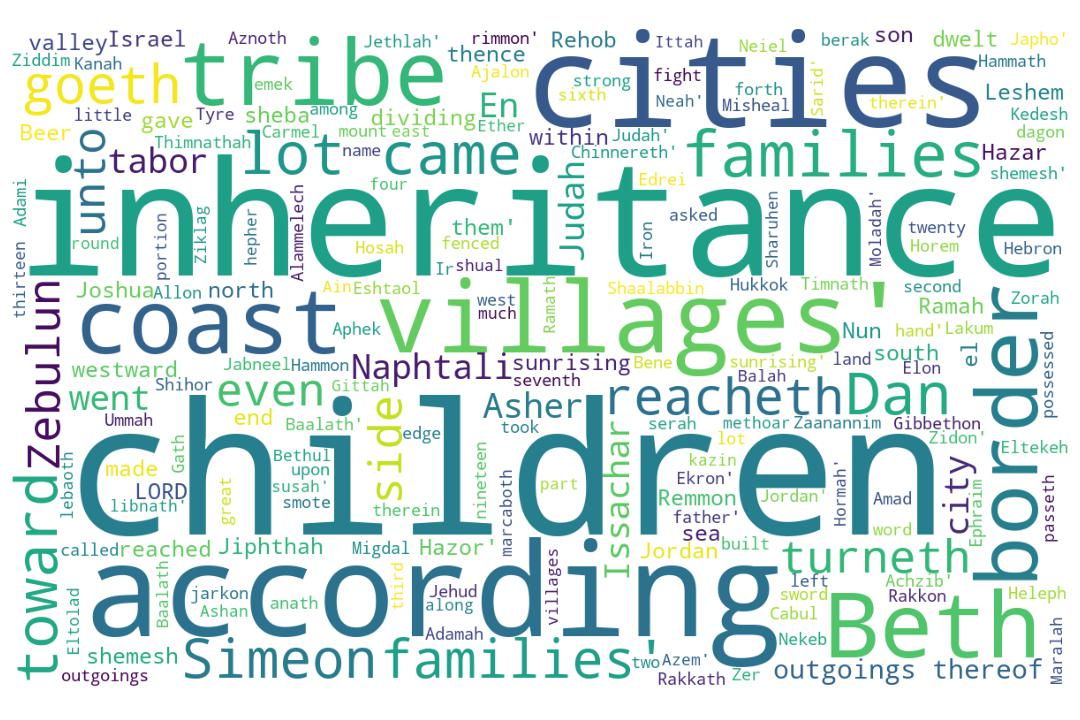
\includegraphics[width=\linewidth]{06OT-Joshua/Joshua19-WordCloud.jpg}
  \caption{Joshua 19 Word Cloud}
  \label{fig:Joshua 19 Word Cloud}
\end{figure}

\marginpar{\scriptsize \centering \fcolorbox{bone}{lime}{\textbf{SIMEON'S PORTION}}\\ (Joshua 19)

\begin{compactenum}[I.][8]

    \item \textbf{Condemned} by Jacob \index[scripture]{Genesis!Gen 34:24--30}(Gen 34:24--30)
    \item \textbf{Cut} out by Moses \index[scripture]{Deuteronomy!Deu 33:08}(Deu 33:8)
    \item To be \textbf{Cast} among Brethren \index[scripture]{Genesis!Gern 49:07}(Gen 49:7)
    \item A Story of \textbf{Carnality} %\index[scripture]{Genesis!Genesis 49:07}(Genesis 49:7)
    \item \textbf{Contained} within Judah \index[scripture]{Joshua!Jsh 19:01}(Jsh 19:1)
    \item A Story of \textbf{Consequences} \index[scripture]{Numbers!Num 25:14}(Num 25:14)

\end{compactenum}}





\footnote{\textcolor[rgb]{0.00,0.25,0.00}{\hyperlink{TOC}{Return to end of Table of Contents.}}}\footnote{\href{https://audiobible.com/bible/joshua_19.html}{\textcolor[cmyk]{0.99998,1,0,0}{Joshua 19 Audio}}}\textcolor[cmyk]{0.99998,1,0,0}{And the second lot came forth to Simeon, \emph{even} for the tribe of the children of Simeon according to their families: and their inheritance was within the inheritance of the children of Judah.}
[2] \textcolor[cmyk]{0.99998,1,0,0}{And they had in their inheritance Beer-sheba, or Sheba, and Moladah,}
[3] \textcolor[cmyk]{0.99998,1,0,0}{And Hazar-shual, and Balah, and Azem,}
[4] \textcolor[cmyk]{0.99998,1,0,0}{And Eltolad, and Bethul, and Hormah,}
[5] \textcolor[cmyk]{0.99998,1,0,0}{And Ziklag, and Beth-marcaboth, and Hazar-susah,}
[6] \textcolor[cmyk]{0.99998,1,0,0}{And Beth-lebaoth, and Sharuhen; thirteen \fcolorbox{bone}{bone}{cities} and their villages:}
[7] \textcolor[cmyk]{0.99998,1,0,0}{Ain, Remmon, and Ether, and Ashan; four \fcolorbox{bone}{bone}{cities} and their villages:}
[8] \textcolor[cmyk]{0.99998,1,0,0}{And all the villages that \emph{were} round about these \fcolorbox{bone}{bone}{cities} to Baalath-beer, Ramath of the south. This \emph{is} the inheritance of the tribe of the children of Simeon according to their families.}
[9] \textcolor[cmyk]{0.99998,1,0,0}{Out of the portion of the children of Judah \emph{was} the inheritance of the children of Simeon: for the part of the children of Judah was too much for them: therefore the children of Simeon had their inheritance within the inheritance of them.}\\
\\
\P \textcolor[cmyk]{0.99998,1,0,0}{And the third lot came up for the children of Zebulun according to their families: and the border of their inheritance was unto Sarid:}
[11] \textcolor[cmyk]{0.99998,1,0,0}{And their border went up toward the sea, and Maralah, and reached to Dabbasheth, and reached to the river that \emph{is} before Jokneam;}
[12] \textcolor[cmyk]{0.99998,1,0,0}{And turned from Sarid eastward toward the sunrising unto the border of Chisloth-tabor, and then goeth out to Daberath, and goeth up to Japhia,}
[13] \textcolor[cmyk]{0.99998,1,0,0}{And from thence passeth on along on the east to Gittah-hepher, to Ittah-kazin, and goeth out to Remmon-methoar to Neah;}
[14] \textcolor[cmyk]{0.99998,1,0,0}{And the border compasseth it on the north side to Hannathon: and the outgoings thereof are in the valley of Jiphthah-el:}
[15] \textcolor[cmyk]{0.99998,1,0,0}{And Kattath, and Nahallal, and Shimron, and Idalah, and Beth-lehem: twelve \fcolorbox{bone}{bone}{cities} with their villages.}
[16] \textcolor[cmyk]{0.99998,1,0,0}{This \emph{is} the inheritance of the children of Zebulun according to their families, these \fcolorbox{bone}{bone}{cities} with their villages.}\\
\\
\P \textcolor[cmyk]{0.99998,1,0,0}{\emph{And} the fourth lot came out to Issachar, for the children of Issachar according to their families.}
[18] \textcolor[cmyk]{0.99998,1,0,0}{And their border was toward Jezreel, and Chesulloth, and Shunem,}
[19] \textcolor[cmyk]{0.99998,1,0,0}{And Haphraim, and Shion, and Anaharath,}
[20] \textcolor[cmyk]{0.99998,1,0,0}{And Rabbith, and Kishion, and Abez,}
[21] \textcolor[cmyk]{0.99998,1,0,0}{And Remeth, and En-gannim, and En-haddah, and Beth-pazzez;}
[22] \textcolor[cmyk]{0.99998,1,0,0}{And the coast reacheth to Tabor, and Shahazimah, and Beth-shemesh; and the outgoings of their border were at Jordan: sixteen \fcolorbox{bone}{bone}{cities} with their villages.}
[23] \textcolor[cmyk]{0.99998,1,0,0}{This \emph{is} the inheritance of the tribe of the children of Issachar according to their families, the \fcolorbox{bone}{bone}{cities} and their villages.}\\
\\
\P \textcolor[cmyk]{0.99998,1,0,0}{And the fifth lot came out for the tribe of the children of Asher according to their families.}
[25] \textcolor[cmyk]{0.99998,1,0,0}{And their border was Helkath, and Hali, and Beten, and Achshaph,}[26] \textcolor[cmyk]{0.99998,1,0,0}{And Alammelech, and Amad, and Misheal; and reacheth to Carmel westward, and to Shihor-libnath;}
[27] \textcolor[cmyk]{0.99998,1,0,0}{And turneth toward the sunrising to Beth-dagon, and reacheth to Zebulun, and to the valley of Jiphthah-el toward the north side of Beth-emek, and Neiel, and goeth out to Cabul on the left hand,}
[28] \textcolor[cmyk]{0.99998,1,0,0}{And Hebron, and Rehob, and Hammon, and Kanah, \emph{even} unto great Zidon;}
[29] \textcolor[cmyk]{0.99998,1,0,0}{And \emph{then} the coast turneth to Ramah, and to the strong city Tyre; and the coast turneth to Hosah; and the outgoings thereof are at the sea from the coast to Achzib:}
[30] \textcolor[cmyk]{0.99998,1,0,0}{Ummah also, and Aphek, and Rehob: twenty and two \fcolorbox{bone}{bone}{cities} with their villages.}
[31] \textcolor[cmyk]{0.99998,1,0,0}{This \emph{is} the inheritance of the tribe of the children of Asher according to their families, these \fcolorbox{bone}{bone}{cities} with their villages.}\\
\\
\P \textcolor[cmyk]{0.99998,1,0,0}{The sixth lot came out to the children of Naphtali, \emph{even} for the children of Naphtali according to their families.}
[33] \textcolor[cmyk]{0.99998,1,0,0}{And their coast was from Heleph, from Allon to Zaanannim, and Adami, Nekeb, and Jabneel, unto Lakum; and the outgoings thereof were at Jordan:}
[34] \textcolor[cmyk]{0.99998,1,0,0}{And \emph{then} the coast turneth westward to Aznoth-tabor, and goeth out from thence to Hukkok, and reacheth to Zebulun on the south side, and reacheth to Asher on the west side, and to Judah upon Jordan toward the sunrising.}
[35] \textcolor[cmyk]{0.99998,1,0,0}{And the fenced \fcolorbox{bone}{bone}{cities} \emph{are} Ziddim, Zer, and Hammath, Rakkath, and Chinnereth,}
[36] \textcolor[cmyk]{0.99998,1,0,0}{And Adamah, and Ramah, and Hazor,}
[37] \textcolor[cmyk]{0.99998,1,0,0}{And Kedesh, and Edrei, and En-hazor,}
[38] \textcolor[cmyk]{0.99998,1,0,0}{And Iron, and Migdal-el, Horem, and Beth-anath, and Beth-shemesh; nineteen \fcolorbox{bone}{bone}{cities} with their villages.}
[39] \textcolor[cmyk]{0.99998,1,0,0}{This \emph{is} the inheritance of the tribe of the children of Naphtali according to their families, the \fcolorbox{bone}{bone}{cities} and their villages.}\\
\\
\P \textcolor[cmyk]{0.99998,1,0,0}{\emph{And} the seventh lot came out for the tribe of the children of Dan according to their families.}
[41] \textcolor[cmyk]{0.99998,1,0,0}{And the coast of their inheritance was Zorah, and Eshtaol, and Ir-shemesh,}
[42] \textcolor[cmyk]{0.99998,1,0,0}{And Shaalabbin, and Ajalon, and Jethlah,}
[43] \textcolor[cmyk]{0.99998,1,0,0}{And Elon, and Thimnathah, and Ekron,}
[44] \textcolor[cmyk]{0.99998,1,0,0}{And Eltekeh, and Gibbethon, and Baalath,}
[45] \textcolor[cmyk]{0.99998,1,0,0}{And Jehud, and Bene-berak, and Gath-rimmon,}
[46] \textcolor[cmyk]{0.99998,1,0,0}{And Me-jarkon, and Rakkon, with the border before Japho.}
[47] \textcolor[cmyk]{0.99998,1,0,0}{And the coast of the children of Dan went out \emph{too} \emph{little} for them: therefore the children of Dan went up to fight against Leshem, and took it, and smote it with the edge of the sword, and possessed it, and dwelt therein, and called Leshem, Dan, after the name of Dan their father.}
[48] \textcolor[cmyk]{0.99998,1,0,0}{This \emph{is} the inheritance of the tribe of the children of Dan according to their families, these \fcolorbox{bone}{bone}{cities} with their villages.}\\
\\
\P \textcolor[cmyk]{0.99998,1,0,0}{When they had made an end of dividing the land for inheritance by their coasts, the children of Israel gave an inheritance to Joshua the son of Nun among them:}
[50] \textcolor[cmyk]{0.99998,1,0,0}{According to the word of the LORD they gave him the city which he asked, \emph{even} Timnath-serah in mount Ephraim: and he built the city, and dwelt therein.}
[51] \textcolor[cmyk]{0.99998,1,0,0}{These \emph{are} the inheritances, which Eleazar the priest, and Joshua the son of Nun, and the heads of the fathers of the tribes of the children of Israel, divided for an inheritance by lot in Shiloh before the LORD, at the door of the tabernacle of the congregation. So they made an end of dividing the country.}
\chapter{Joshua 20}


% \textcolor[cmyk]{0.99998,1,0,0}{
\marginpar{\scriptsize \centering \fcolorbox{bone}{lime}{\textbf{CITIES OF REFUGE}}\\ (Joshua 20)

\begin{compactenum}[I.][8]

    \item \textbf{Presumptions}  \index[scripture]{Joshua!Jsh 20:03}(Jsh 20:3)
    \item \textbf{Persons} Killed \index[scripture]{Joshua!Jsh 20:03} \index[scripture]{Joshua!Jsh 20:09} (Jsh 20:3, 9)
    \item A \textbf{Place} of Refuge \index[scripture]{Joshua!Jsh 20:04}(Jsh 20:4)
    \item Being \textbf{Pursued}  \index[scripture]{Joshua!Jsh 20:05}(Jsh 20:5)
    \item The \textbf{Life} of the Priest \index[scripture]{Joshua!Jsh 20:06}(Jsh 20:6)
    \item The \textbf{Plain} of Reuben \index[scripture]{Joshua!Jsh 20:08}(Jsh 20:8)
   \item \textbf{Protection}  %\index[scripture]{Joshua!Jsh 20:03}(Jsh 20:3)

\end{compactenum}}





\footnote{\textcolor[rgb]{0.00,0.25,0.00}{\hyperlink{TOC}{Return to end of Table of Contents.}}}\footnote{\href{https://audiobible.com/bible/joshua_20.html}{\textcolor[cmyk]{0.99998,1,0,0}{Joshua 20 Audio}}}\textcolor[cmyk]{0.99998,1,0,0}{The LORD also spake unto Joshua, saying,}
[2] \textcolor[cmyk]{0.99998,1,0,0}{Speak to the children of Israel, saying, Appoint out for you cities of refuge, whereof I spake unto you by the hand of Moses:}
[3] \textcolor[cmyk]{0.99998,1,0,0}{That the slayer that killeth \emph{any} person unawares \emph{and} unwittingly may flee thither: and they shall be your refuge from the avenger of blood.}
[4] \textcolor[cmyk]{0.99998,1,0,0}{And when he that doth flee unto one of those cities shall stand at the entering of the gate of the city, and shall declare his cause in the ears of the elders of that city, they shall take him into the city unto them, and give him a place, that he may dwell among them.}
[5] \textcolor[cmyk]{0.99998,1,0,0}{And if the avenger of blood pursue after him, then they shall not deliver the slayer up into his hand; because he smote his neighbour unwittingly, and hated him not beforetime.}
[6] \textcolor[cmyk]{0.99998,1,0,0}{And he shall dwell in that city, until he stand before the congregation for judgment, \emph{and} until the death of the high priest that shall be in those days: then shall the slayer return, and come unto his own city, and unto his own house, unto the city from whence he fled.}\\
\\
\P \textcolor[cmyk]{0.99998,1,0,0}{And they appointed Kedesh in Galilee in mount Naphtali, and Shechem in mount Ephraim, and Kirjath-arba, which \emph{is} Hebron, in the mountain of Judah.}
[8] \textcolor[cmyk]{0.99998,1,0,0}{And on the other side Jordan by Jericho eastward, they assigned Bezer in the wilderness upon the plain out of the tribe of Reuben, and Ramoth in Gilead out of the tribe of Gad, and Golan in Bashan out of the tribe of Manasseh.}
[9] \textcolor[cmyk]{0.99998,1,0,0}{These were the cities appointed for all the children of Israel, and for the stranger that sojourneth among them, that whosoever killeth \emph{any} person at unawares might flee thither, and not die by the hand of the avenger of blood, until he stood before the congregation.}
\chapter{Joshua 21}

\begin{figure}
  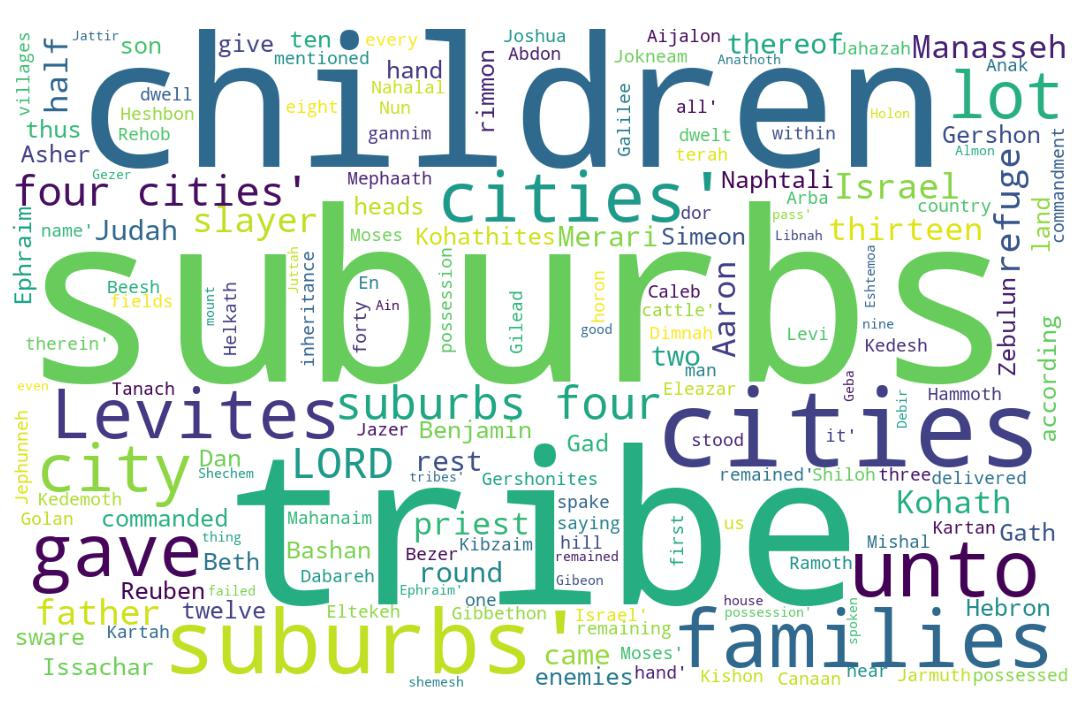
\includegraphics[width=\linewidth]{06OT-Joshua/Joshua21-WordCloud.jpg}
  \caption{Joshua 21 Word Cloud}
  \label{fig:Joshua 21 Word Cloud}
\end{figure}

\marginpar{\scriptsize \centering \fcolorbox{bone}{lime}{\textbf{CITIES FOR THE LEVITES}}\\ (Joshua 21)

\begin{compactenum}[I.][8]

    \item The \textbf{Priests} \index[scripture]{Joshua!Jsh 21:01}\index[scripture]{Joshua!Jsh 21:04}\index[scripture]{Joshua!Jsh 21:13}\index[scripture]{Joshua!Jsh 21:19}  (Jsh 21:1, 4, 13, 19)
    \item A \textbf{Place} Set Aside %\index[scripture]{Joshua!Jsh 21:04} (Jsh 21:4)
    \item The \textbf{Appointing} \index[scripture]{Joshua!Jsh 21:04} (Jsh 21:4)
    \item \textbf{Pastures} \index[scripture]{Joshua!Jsh 21:09}\index[scripture]{Joshua!Jsh 21:42} (Jsh 21:9, 42)
    \item Took \textbf{Possession} \index[scripture]{Joshua!Jsh 21:12} \index[scripture]{Joshua!Jsh 21:41}  \index[scripture]{Joshua!Jsh 21:43} (Jsh 21:12, 41, 43)
    \item God's Word Come to Pass  \index[scripture]{Joshua!Jsh 21:45}  (Jsh 21:45)

\end{compactenum}}





\footnote{\textcolor[rgb]{0.00,0.25,0.00}{\hyperlink{TOC}{Return to end of Table of Contents.}}}\footnote{\href{https://audiobible.com/bible/joshua_21.html}{\textcolor[cmyk]{0.99998,1,0,0}{Joshua 21 Audio}}}\textcolor[cmyk]{0.99998,1,0,0}{Then came near the heads of the fathers of the Levites unto Eleazar the priest, and unto Joshua the son of Nun, and unto the heads of the fathers of the tribes of the children of Israel;}
[2] \textcolor[cmyk]{0.99998,1,0,0}{And they spake unto them at Shiloh in the land of Canaan, saying, The LORD commanded by the hand of Moses to give us cities to dwell in, with the suburbs thereof for our cattle.}
[3] \textcolor[cmyk]{0.99998,1,0,0}{And the children of Israel gave unto the Levites out of their inheritance, at the commandment of the LORD, these cities and their suburbs.}
[4] \textcolor[cmyk]{0.99998,1,0,0}{And the lot came out for the families of the Kohathites: and the children of Aaron the priest, \emph{which} \emph{were} of the Levites, had by lot out of the tribe of Judah, and out of the tribe of Simeon, and out of the tribe of Benjamin, thirteen cities.}
[5] \textcolor[cmyk]{0.99998,1,0,0}{And the rest of the children of Kohath \emph{had} by lot out of the families of the tribe of Ephraim, and out of the tribe of Dan, and out of the half tribe of Manasseh, ten cities.}
[6] \textcolor[cmyk]{0.99998,1,0,0}{And the children of Gershon \emph{had} by lot out of the families of the tribe of Issachar, and out of the tribe of Asher, and out of the tribe of Naphtali, and out of the half tribe of Manasseh in Bashan, thirteen cities.}
[7] \textcolor[cmyk]{0.99998,1,0,0}{The children of Merari by their families \emph{had} out of the tribe of Reuben, and out of the tribe of Gad, and out of the tribe of Zebulun, twelve cities.}
[8] \textcolor[cmyk]{0.99998,1,0,0}{And the children of Israel gave by lot unto the Levites these cities with their suburbs, as the LORD commanded by the hand of Moses.}\\
\\
\P \textcolor[cmyk]{0.99998,1,0,0}{And they gave out of the tribe of the children of Judah, and out of the tribe of the children of Simeon, these cities which are \emph{here} mentioned by name,}
[10] \textcolor[cmyk]{0.99998,1,0,0}{Which the children of Aaron, \emph{being} of the families of the Kohathites, \emph{who} \emph{were} of the children of Levi, had: for their's was the first lot.}
[11] \textcolor[cmyk]{0.99998,1,0,0}{And they gave them the city of Arba the father of Anak, which \emph{city} \emph{is} Hebron, in the hill \emph{country} of Judah, with the suburbs thereof round about it.}
[12] \textcolor[cmyk]{0.99998,1,0,0}{But the fields of the city, and the villages thereof, gave they to Caleb the son of Jephunneh for his possession.}\\
\\
\P \textcolor[cmyk]{0.99998,1,0,0}{Thus they gave to the children of Aaron the priest Hebron with her suburbs, \emph{to} \emph{be} a city of refuge for the slayer; and Libnah with her suburbs,}
[14] \textcolor[cmyk]{0.99998,1,0,0}{And Jattir with her suburbs, and Eshtemoa with her suburbs,}
[15] \textcolor[cmyk]{0.99998,1,0,0}{And Holon with her suburbs, and Debir with her suburbs,}
[16] \textcolor[cmyk]{0.99998,1,0,0}{And Ain with her suburbs, and Juttah with her suburbs, \emph{and} Beth-shemesh with her suburbs; nine cities out of those two tribes.}
[17] \textcolor[cmyk]{0.99998,1,0,0}{And out of the tribe of Benjamin, Gibeon with her suburbs, Geba with her suburbs,}
[18] \textcolor[cmyk]{0.99998,1,0,0}{Anathoth with her suburbs, and Almon with her suburbs; four cities.}
[19] \textcolor[cmyk]{0.99998,1,0,0}{All the cities of the children of Aaron, the priests, \emph{were} thirteen cities with their suburbs.}\\
\\
\P \textcolor[cmyk]{0.99998,1,0,0}{And the families of the children of Kohath, the Levites which remained of the children of Kohath, even they had the cities of their lot out of the tribe of Ephraim.}
[21] \textcolor[cmyk]{0.99998,1,0,0}{For they gave them Shechem with her suburbs in mount Ephraim, \emph{to} \emph{be} a city of refuge for the slayer; and Gezer with her suburbs,}
[22] \textcolor[cmyk]{0.99998,1,0,0}{And Kibzaim with her suburbs, and Beth-horon with her suburbs; four cities.}
[23] \textcolor[cmyk]{0.99998,1,0,0}{And out of the tribe of Dan, Eltekeh with her suburbs, Gibbethon with her suburbs,}
[24] \textcolor[cmyk]{0.99998,1,0,0}{Aijalon with her suburbs, Gath-rimmon with her suburbs; four cities.}
[25] \textcolor[cmyk]{0.99998,1,0,0}{And out of the half tribe of Manasseh, Tanach with her suburbs, and Gath-rimmon with her suburbs; two cities.}
[26] \textcolor[cmyk]{0.99998,1,0,0}{All the cities \emph{were} ten with their suburbs for the families of the children of Kohath that remained.}\\
\\
\P \textcolor[cmyk]{0.99998,1,0,0}{And unto the children of Gershon, of the families of the Levites, out of the \emph{other} half tribe of Manasseh \emph{they} \emph{gave} Golan in Bashan with her suburbs, \emph{to} \emph{be} a city of refuge for the slayer; and Beesh-terah with her suburbs; two cities.}
[28] \textcolor[cmyk]{0.99998,1,0,0}{And out of the tribe of Issachar, Kishon with her suburbs, Dabareh with her suburbs,}
[29] \textcolor[cmyk]{0.99998,1,0,0}{Jarmuth with her suburbs, En-gannim with her suburbs; four cities.}
[30] \textcolor[cmyk]{0.99998,1,0,0}{And out of the tribe of Asher, Mishal with her suburbs, Abdon with her suburbs,}
[31] \textcolor[cmyk]{0.99998,1,0,0}{Helkath with her suburbs, and Rehob with her suburbs; four cities.}
[32] \textcolor[cmyk]{0.99998,1,0,0}{And out of the tribe of Naphtali, Kedesh in Galilee with her suburbs, \emph{to} \emph{be} a city of refuge for the slayer; and Hammoth-dor with her suburbs, and Kartan with her suburbs; three cities.}
[33] \textcolor[cmyk]{0.99998,1,0,0}{All the cities of the Gershonites according to their families \emph{were} thirteen cities with their suburbs.}\\
\\
\P \textcolor[cmyk]{0.99998,1,0,0}{And unto the families of the children of Merari, the rest of the Levites, out of the tribe of Zebulun, Jokneam with her suburbs, and Kartah with her suburbs,}
[35] \textcolor[cmyk]{0.99998,1,0,0}{Dimnah with her suburbs, Nahalal with her suburbs; four cities.}
[36] \textcolor[cmyk]{0.99998,1,0,0}{And out of the tribe of Reuben, Bezer with her suburbs, and Jahazah with her suburbs,}
[37] \textcolor[cmyk]{0.99998,1,0,0}{Kedemoth with her suburbs, and Mephaath with her suburbs; four cities.}
[38] \textcolor[cmyk]{0.99998,1,0,0}{And out of the tribe of Gad, Ramoth in Gilead with her suburbs, \emph{to} \emph{be} a city of refuge for the slayer; and Mahanaim with her suburbs,}
[39] \textcolor[cmyk]{0.99998,1,0,0}{Heshbon with her suburbs, Jazer with her suburbs; four cities in all.}\\
\\
\P \textcolor[cmyk]{0.99998,1,0,0}{And the LORD gave unto Israel all the land which he sware to give unto their fathers; and they possessed it, and dwelt therein.}
[44] \textcolor[cmyk]{0.99998,1,0,0}{And the LORD gave them rest round about, according to all that he sware unto their fathers: and there stood not a man of all their enemies before them; the LORD delivered all their enemies into their hand.}
[45] \textcolor[cmyk]{0.99998,1,0,0}{There failed not ought of any good thing which the LORD had spoken unto the house of Israel; all came to pass.}

\chapter{Psalm 71}

\begin{figure}
  \includegraphics[width=\linewidth]{19OT-Psalms/Psalm71-wordcloud.jpg}
  \caption{Psalm 71 Word Cloud}
  \label{fig:Psalm 71 word Cloud}
\end{figure}

\marginpar{\scriptsize \centering \fcolorbox{bone}{lime}{\textbf{THE LORD MY TRUST}}\\ (Psalm 71:1-24) \begin{compactenum}[I.][8]
     \item My \textbf{Cry} \index[scripture]{Psalms!Psa 071:02}(Psa 71:2)
    \item God's \textbf{Commandment} to save me \index[scripture]{Psalms!Psa 071:03}(Psa 71:3)
    \item My \textbf{Confidence} \index[scripture]{Psalms!Psa 071:05}(Psa 71:5)
    \item My \textbf{Continuance} \index[scripture]{Psalms!Psa 071:06}\index[scripture]{Psalms!Psa 071:14} (Psa 71:6, 14)
    \item Evil \textbf{Counsel} \index[scripture]{Psalms!Psa 071:10}(Psa 71:10)
    \item Eternal \textbf{Covering} for the wicked \index[scripture]{Psalms!Psa 071:13}(Psa 71:13)
    \item Enemy \textbf{Confounding} \index[scripture]{Psalms!Psa 071:24}(Psa 71:24)
\end{compactenum}}

\footnote{\textcolor[cmyk]{0.99998,1,0,0}{\hyperlink{TOC}{Return to end of Table of Contents.}}}\footnote{\href{https://audiobible.com/bible/psalms_71.html}{\textcolor[cmyk]{0.99998,1,0,0}{Psalm 71 Audio}}}\textcolor[cmyk]{0.99998,1,0,0}{In thee, O LORD, do I put my trust: let me never be put to confusion.}
[2] \textcolor[cmyk]{0.99998,1,0,0}{\fcolorbox{bone}{lime}{Deliver me} in thy \fcolorbox{bone}{MYGOLD}{righteousness}, and \fcolorbox{bone}{lime}{cause me} to escape: \fcolorbox{bone}{lime}{incline thine ear} unto me, and save me.}
[3] \textcolor[cmyk]{0.99998,1,0,0}{Be thou my strong habitation, whereunto I may continually resort: thou hast given commandment \fcolorbox{bone}{lime}{to save me}; for thou \emph{art} my rock and my fortress.}
[4] \textcolor[cmyk]{0.99998,1,0,0}{Deliver me, O my God, out \fcolorbox{bone}{bone}{of} the hand \fcolorbox{bone}{bone}{of} the wicked, out \fcolorbox{bone}{bone}{of} the hand \fcolorbox{bone}{bone}{of}  the unrighteous and cruel man.}
[5] \textcolor[cmyk]{0.99998,1,0,0}{For thou \emph{art} \fcolorbox{bone}{lime}{my hope}, O Lord GOD: \emph{thou} \emph{art} \fcolorbox{bone}{lime}{my trust} from my youth.}
[6] \textcolor[cmyk]{0.99998,1,0,0}{By thee have I been holden up from the womb: thou art he that took me out \fcolorbox{bone}{bone}{of}   my mother's bowels: my praise \emph{shall} \emph{be} \fcolorbox{bone}{lime}{continually} \fcolorbox{bone}{bone}{of}   thee.}
[7] \textcolor[cmyk]{0.99998,1,0,0}{I am as a wonder unto many; but thou \emph{art} my strong refuge.}
[8] \textcolor[cmyk]{0.99998,1,0,0}{Let my mouth be filled \emph{with} thy praise \emph{and} \emph{with} thy honour all the day.}
[9] \textcolor[cmyk]{0.99998,1,0,0}{Cast me not off in the time \fcolorbox{bone}{bone}{of}   old age; forsake me not when my strength faileth.}
[10] \textcolor[cmyk]{0.99998,1,0,0}{For mine enemies speak against me; and they that lay wait for my soul take \fcolorbox{bone}{lime}{counsel} together,}
[11] \textcolor[cmyk]{0.99998,1,0,0}{Saying, God hath forsaken him: persecute and take him; for \emph{there} \emph{is} none to deliver \emph{him}.}
[12] \textcolor[cmyk]{0.99998,1,0,0}{O God, be not far from me: O my God, make haste for my help.}
[13] \textcolor[cmyk]{0.99998,1,0,0}{Let them be \fcolorbox{bone}{lime}{confounded} \emph{and} \fcolorbox{bone}{lime}{consumed} that are adversaries to my soul; let them be \fcolorbox{bone}{lime}{covered} \emph{with} reproach and dishonour that seek my hurt.}%\marginpar{\scriptsize \textcolor[rgb]{0.00,0.545,0.269}
%{$\rightarrow$1. Confounded, 2. Consumed, 3. Covered
%\begin{compactenum}
%	\item A proud look,
%	\item a lying tongue,
%	\item hands that shed innocent blood,
%	\item An heart that deviseth wicked imaginations,
%	\item feet that be swift in running to mischief,
%	\item A false witness that speaketh lies, and
%	\item he that soweth discord among brethren.
%\end{compactenum}
%}
%} 
[14] \textcolor[cmyk]{0.99998,1,0,0}{But I will hope continually, and will yet praise thee more and more.}
[15] \textcolor[cmyk]{0.99998,1,0,0}{My mouth shall shew forth thy \fcolorbox{bone}{MYGOLD}{righteousness} \emph{and} thy salvation all the day; for I know not the numbers \emph{thereof}.}
[16] \textcolor[cmyk]{0.99998,1,0,0}{I will go in the strength \fcolorbox{bone}{bone}{of}  the Lord GOD: I will make mention \fcolorbox{bone}{bone}{of}  thy \fcolorbox{bone}{MYGOLD}{righteousness}, \emph{even} \fcolorbox{bone}{bone}{of}  thine only.}
[17] \textcolor[cmyk]{0.99998,1,0,0}{O God, thou hast taught me from my youth: and hitherto have I declared thy wondrous works.}
[18] \textcolor[cmyk]{0.99998,1,0,0}{Now also when I am old and grayheaded, O God, forsake me not; until I have shewed thy strength unto \emph{this} generation, \emph{and} thy power to every one \emph{that} is to come.}
[19] \textcolor[cmyk]{0.99998,1,0,0}{Thy \fcolorbox{bone}{MYGOLD}{righteousness} also, O God, \emph{is} very high, who hast done great things: O God, who \emph{is} like unto thee!}
[20] \textcolor[cmyk]{0.99998,1,0,0}{\emph{Thou}, which hast shewed me great and sore troubles, shalt quicken me again, and shalt bring me up again from the depths \fcolorbox{bone}{bone}{of}  the earth.}
[21] \textcolor[cmyk]{0.99998,1,0,0}{Thou shalt increase my greatness, and comfort me on every side.}
[22] \textcolor[cmyk]{0.99998,1,0,0}{I will also praise thee with the psaltery, \emph{even} thy truth, O my God: unto thee will I sing with the harp, O thou Holy One \fcolorbox{bone}{bone}{of}  Israel.}
[23] \textcolor[cmyk]{0.99998,1,0,0}{My lips shall greatly rejoice when I sing unto thee; and my soul, which thou hast redeemed.}
[24] \textcolor[cmyk]{0.99998,1,0,0}{My tongue also shall talk \fcolorbox{bone}{bone}{of}  thy \fcolorbox{bone}{MYGOLD}{righteousness} all the day long: for they are \fcolorbox{bone}{lime}{confounded}, for they are brought unto shame, that seek my hurt.}

\chapter{Proverb 12}

\begin{figure}
  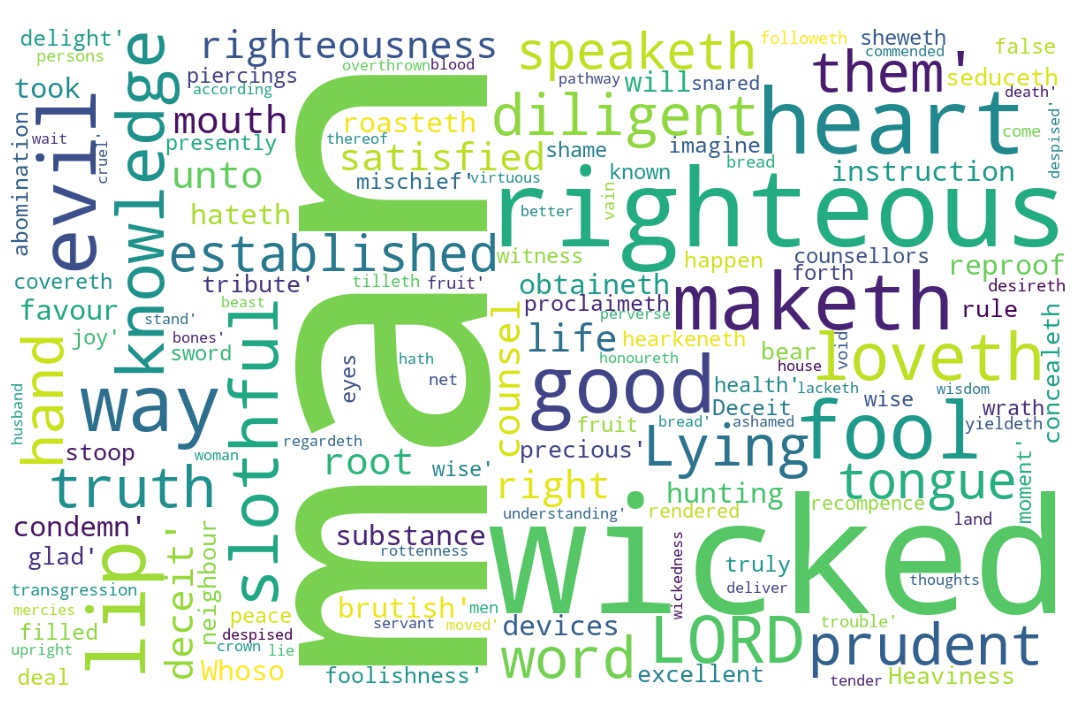
\includegraphics[width=\linewidth]{20OT-Proverbs/Proverb12-WordCloud.jpg}
  \caption{Proverb 12 Word Cloud}
  \label{fig:Proverb 12 Word Cloud}
\end{figure}

\marginpar{\scriptsize \centering \fcolorbox{bone}{lime}{\textbf{SURE THINGS}}\\ (Proverb 12:1-27) \begin{compactenum}[I.][8]
    \item \textbf{Contented Man} \index[scripture]{Proverbs!Pro 12:01}(Pro 12:1) 
    \item \textbf{Contentious Mate} \index[scripture]{Proverbs!Pro 12:04}(Pro 12:4) 
    \item \textbf{Commended Man} \index[scripture]{Proverbs!Pro 12:08}(Pro 12:8) 
    \item \textbf{Condemned Man} \index[scripture]{Proverbs!Pro 12:09}(Pro 12:9) 
    \item \textbf{Correct Mouth} \index[scripture]{Proverbs!Pro 12:17}(Pro 12:17) 
    \item \textbf{Continual Misery} \index[scripture]{Proverbs!Pro 12:25}(Pro 12:25) 
    \item \textbf{Comforting Materials} \index[scripture]{Proverbs!Pro 12:27}(Pro 12:27) 
\end{compactenum}}

\marginpar{\scriptsize \centering \fcolorbox{bone}{yellow}{\textbf{WICKED WAYS \& WORDS}}\\ (Proverb 12:1-27) \begin{compactenum}[I.][8]
    \item They do not Provide \textbf{Security} \index[scripture]{Proverbs!Pro 12:03}(Pro 12:3) 
    \item They do not Provide \textbf{Satisfaction} \index[scripture]{Proverbs!Pro 12:11}\index[scripture]{Proverbs!Pro 12:14}(Pro 12:11, 14) 
    \item They are \textbf{Snares} \index[scripture]{Proverbs!Pro 12:13}(Pro 12:13) 
    \item They lead to \textbf{Shame} \index[scripture]{Proverbs!Pro 12:16}(Pro 12:16) 
    \item They Pierce like a \textbf{Sword} \index[scripture]{Proverbs!Pro 12:18}(Pro 12:18) 
    \item They Produce \textbf{Slothfulness and Servanthood} \index[scripture]{Proverbs!Pro 12:24}\index[scripture]{Proverbs!Pro 12:27}(Prov 12:24, 27) 
\end{compactenum}}

\marginpar{\scriptsize \centering \fcolorbox{bone}{black}{\textbf{\textcolor[cmyk]{0,0,0,0}{PARTS OF LIFE}}}\\ (Proverb 12:1-27) 
 \begin{compactenum}[I.][8]
    \item \textbf{Path to Growth} \index[scripture]{Proverbs!Pro 12:01}(Pro 12:1) 
    \item \textbf{Promise of God} \index[scripture]{Proverbs!Pro 12:02} (Pro 12:2) 
    \item \textbf{Perennial Aggravation} \index[scripture]{Proverbs!Pro 12:04}(Pro 12:04)
    \item \textbf{Perverse Goals} \index[scripture]{Proverbs!Pro 12:08}(Pro 12:08) 
    \item \textbf{Presence of Grief} \index[scripture]{Proverbs!Pro 12:08}(Pro 12:08)
    \item \textbf{Practical Regard} \index[scripture]{Proverbs!Pro 12:10}(Pro 12:10) 
    \item \textbf{Pattern of Goodness} \index[scripture]{Proverbs!Pro 12:24}(Pro 12:24) 
\end{compactenum}}


\marginpar{\scriptsize \centering \fcolorbox{bone}{blue}{\textbf{\textcolor[cmyk]{0,0,0,0}{A VIRTUOUS WOMAN}}}\\ (Proverb 12:1-27) 
 \begin{compactenum}[I.][8]
    \item \textbf{Correctable} \index[scripture]{Proverbs!Pro 12:04}(Pro 12:4) 
    \item \textbf{Conformable} \index[scripture]{Proverbs!Pro 12:04}(Pro 12:4) 
    \item \textbf{Cooperative} \index[scripture]{Proverbs!Pro 12:04}(Pro 12:4) 
    \item \textbf{Calm} \index[scripture]{Proverbs!Pro 12:04}(Pro 12:4) 
    \item A \textbf{Crown} \index[scripture]{Proverbs!Pro 12:04}(Pro 12:4) 
    \item \textbf{Caring} \index[scripture]{Proverbs!Pro 12:04}(Pro 12:4) 
    \item \textbf{Considerate} \index[scripture]{Proverbs!Pro 12:04}(Pro 12:4) 
\end{compactenum}}

\marginpar{\scriptsize \centering \fcolorbox{bone}{orange}{\textbf{THE EXAMINATION}}\\ (Proverb 12:1-27) \begin{compactenum}[I.][8]
    \item What their \textbf{Hearts} Love \index[scripture]{Proverbs!Pro 12:01}(Pro 12:1) 
    \item What Their \textbf{Hands} Produce \index[scripture]{Proverbs!Pro 12:04}(Pro 12:4) 
    \item \textbf{How} they treat the Helpless \index[scripture]{Proverbs!Pro 12:08}(Pro 12:8) 
    \item The \textbf{Health} of Their speech \index[scripture]{Proverbs!Pro 12:181}(Pro 12:8) 
    \item What he \textbf{Hearkened} to \index[scripture]{Proverbs!Pro 12:15}(Pro 12:15) 
    \item What is \textbf{Honoured} to \index[scripture]{Proverbs!Pro 12:09}(Pro 12:9) 
    \item How they \textbf{Handle} the Details
    \index[scripture]{Proverbs!Pro 12:09}(Pro 12:9) 
\end{compactenum}}

%%%%%%%%%%%%%%%%%%%%%%%%%%%%%%%%%%
%%%%%%%%%%%%%%%%%%%%%%%%%%%%%%%%%
\footnote{\textcolor[cmyk]{0.99998,1,0,0}{\hyperlink{TOC}{Return to end of Table of Contents.}}}\footnote{\href{https://audiobible.com/bible/proverbs_12.html}{\textcolor[cmyk]{0.99998,1,0,0}{Proverbs Audio}}}\textcolor[cmyk]{0.99998,1,0,0}{Whoso \fcolorbox{bone}{lime}{loveth instruction} loveth \fcolorbox{bone}{blue}{\textbf{\textcolor[cmyk]{0,0,0,0}{knowledge}}}: but he that hateth reproof \emph{is} brutish.}
[2] \textcolor[cmyk]{0.99998,1,0,0}{A good \emph{man} obtaineth \fcolorbox{bone}{lime}{favour of} \fcolorbox{bone}{blue}{\textbf{\textcolor[cmyk]{0,0,0,0}{the LORD}}}: but \fcolorbox{bone}{bone}{a} man of wicked devices will he condemn.}
[3] \textcolor[cmyk]{0.99998,1,0,0}{A man shall \fcolorbox{bone}{yellow}{not be}  \fcolorbox{bone}{yellow}{established} by wickedness: but the root of the righteous shall not be moved.}
[4] \textcolor[cmyk]{0.99998,1,0,0}{A virtuous woman \emph{is} \fcolorbox{bone}{bone}{a} crown to her husband: but she that maketh ashamed \emph{is} as \fcolorbox{bone}{blue}{\textbf{\textcolor[cmyk]{0,0,0,0}{rottenness in his bones}}}.}
[5] \textcolor[cmyk]{0.99998,1,0,0}{The thoughts of the righteous \emph{are} right: \emph{but} the counsels of the wicked \emph{are} deceit.}
[6] \textcolor[cmyk]{0.99998,1,0,0}{The words of the wicked \emph{are} to lie in wait for blood: but the mouth of the upright shall deliver them.}
[7] \textcolor[cmyk]{0.99998,1,0,0}{The wicked are overthrown, and \emph{are} not: but the house of the righteous shall stand.}
[8] \textcolor[cmyk]{0.99998,1,0,0}{A man shall be \fcolorbox{bone}{lime}{commended} according to his wisdom: but he that is of \fcolorbox{bone}{bone}{a} \fcolorbox{bone}{blue}{\textbf{\textcolor[cmyk]{0,0,0,0}{perverse}}} heart shall be despised.}
[9] \textcolor[cmyk]{0.99998,1,0,0}{\emph{He} \emph{that} \emph{is} \fcolorbox{bone}{lime}{despised}, and hath \fcolorbox{bone}{bone}{a} servant, \emph{is} better than he that honoureth himself, and lacketh bread.}
[10] \textcolor[cmyk]{0.99998,1,0,0}{A righteous \emph{man} \fcolorbox{bone}{blue}{\textbf{\textcolor[cmyk]{0,0,0,0}{regardeth}}} the life of his beast: but the tender mercies of the wicked \emph{are} cruel.}
[11] \textcolor[cmyk]{0.99998,1,0,0}{He that tilleth his land shall be \fcolorbox{bone}{yellow}{satisfied} with bread: but he that followeth vain \emph{persons} \emph{is} void of \fcolorbox{bone}{MYGOLD}{understanding}.}
[12] \textcolor[cmyk]{0.99998,1,0,0}{The wicked desireth the net of evil \emph{men}: but the root of the righteous yieldeth \emph{fruit}.}
[13] \textcolor[cmyk]{0.99998,1,0,0}{The wicked is \fcolorbox{bone}{yellow}{snared} by the \fcolorbox{bone}{MYGOLD}{transgression} of \emph{his} lips: but the just shall come out of trouble.}\footnote{\textbf{Ecclesiastes 9:12} - For man also knoweth not his time: as the fishes that are taken in an evil net, and as the birds that are caught in the snare; so are the sons of men snared in an evil time, when it falleth suddenly upon them.}\footnote{\textbf{Isaiah 28:13} - But the word of the LORD was unto them precept upon precept, precept upon precept; line upon line, line upon line; here a little, and there a little; that they might go, and fall backward, and be broken, and snared, and taken.}\footnote{\textbf{Isaiah 42:22} - But this is a people robbed and spoiled; they are all of them snared in holes, and they are hid in prison houses: they are for a prey, and none delivereth; for a spoil, and none saith, Restore.}
[14] \textcolor[cmyk]{0.99998,1,0,0}{A man shall be satisfied with good by the fruit of \emph{his} mouth: and the recompence of \fcolorbox{bone}{bone}{a} man's hands shall be rendered unto him.}
[15] \textcolor[cmyk]{0.99998,1,0,0}{The way of \fcolorbox{bone}{bone}{a} fool \emph{is} right in his own eyes: but he that hearkeneth unto counsel \emph{is} wise.}
[16] \textcolor[cmyk]{0.99998,1,0,0}{A fool's wrath is presently known: but \fcolorbox{bone}{bone}{a} prudent \emph{man} covereth \fcolorbox{bone}{yellow}{shame}.}\footnote{\textbf{Proverb 27:3}  -  A stone is heavy, and the sand weighty; but a fool’s wrath is heavier than them both.}
[17] \textcolor[cmyk]{0.99998,1,0,0}{\emph{He} \emph{that} \fcolorbox{bone}{lime}{speaketh truth} sheweth forth \fcolorbox{bone}{MYGOLD}{righteousness}: but \fcolorbox{bone}{bone}{a} false witness deceit.}
[18] \textcolor[cmyk]{0.99998,1,0,0}{There is that speaketh like the piercings of \fcolorbox{bone}{bone}{a} \fcolorbox{bone}{yellow}{sword}: but the tongue of the wise \emph{is} health.}
[19] \textcolor[cmyk]{0.99998,1,0,0}{The lip of truth shall be established for ever: but \fcolorbox{bone}{bone}{a} lying tongue \emph{is} but for \fcolorbox{bone}{bone}{a} moment.}
[20] \textcolor[cmyk]{0.99998,1,0,0}{Deceit \emph{is} in the heart of them that imagine evil: but to the counsellors of peace \emph{is} joy.}
[21] \textcolor[cmyk]{0.99998,1,0,0}{There shall no evil happen to the just: but the wicked shall be filled with mischief.}
[22] \textcolor[cmyk]{0.99998,1,0,0}{Lying lips \emph{are} abomination to the LORD: but they that deal truly \emph{are} his delight.}
[23] \textcolor[cmyk]{0.99998,1,0,0}{A prudent man concealeth knowledge: but the heart of fools proclaimeth foolishness.}
[24] \textcolor[cmyk]{0.99998,1,0,0}{\fcolorbox{bone}{blue}{\textbf{\textcolor[cmyk]{0,0,0,0}{The hand of the diligent}}} shall bear rule: but the \fcolorbox{bone}{yellow}{slothful} shall be under \fcolorbox{bone}{yellow}{tribute.}}
[25] \textcolor[cmyk]{0.99998,1,0,0}{\fcolorbox{bone}{lime}{Heaviness} in the heart of man maketh it stoop: but \fcolorbox{bone}{bone}{a} good word maketh it glad.}
[26] \textcolor[cmyk]{0.99998,1,0,0}{The righteous \emph{is} more excellent than his neighbour: but the way of the wicked seduceth them.}
[27] \textcolor[cmyk]{0.99998,1,0,0}{The \fcolorbox{bone}{yellow}{slothful} \emph{man} roasteth not that which he took in hunting: but the substance of \fcolorbox{bone}{bone}{a} diligent man \emph{is} \fcolorbox{bone}{lime}{precious}.}
[28] \textcolor[cmyk]{0.99998,1,0,0}{In the way of \fcolorbox{bone}{MYGOLD}{righteousness} \emph{is} life; and \emph{in} the pathway \emph{thereof} \emph{there} \emph{is} no death.}\footnote{\textbf{Psalm 1:1, 6} - Blessed is the man that walketh not in the counsel of the ungodly, nor standeth in the way of sinners, nor sitteth in the seat of the scornful. [6] For the LORD knoweth the way of the righteous: but the way of the ungodly shall perish.}






\end{document}

